\documentclass[CJK,notheorems,mathserif,table]{beamer}
\useoutertheme[height=0.1\textwidth,width=0.15\textwidth,hideothersubsections]{sidebar}
\usecolortheme{whale}      % Outer color themes, 其他选择: whale, seahorse, dolphin . 换一个编译看看有什么不同.
\usecolortheme{orchid}     % Inner color themes, 其他选择: lily, orchid
\useinnertheme[shadow]{rounded} % 对 box 的设置: 圆角、有阴影.
\setbeamercolor{sidebar}{bg=blue!60} % sidebar的颜色, 50%的蓝色.
%\setbeamercolor{background canvas}{bg=blue!9} % 背景色, 9%的蓝色. 去掉下一行, 试一试这个.
\setbeamertemplate{background canvas}[vertical shading][bottom=white,top=structure.fg!25] %%背景色, 上25%的蓝, 过渡到下白.
\usefonttheme{serif}  % 字体. 个人偏好有轮廓的字体. 去掉这个设置编译, 就看到不同了.
\setbeamertemplate{navigation symbols}{}   %% 去掉页面下方默认的导航条.
%%------------------------常用宏包---------------------------------------------------------------------
%%注意, beamer 会默认使用下列宏包: amsthm, graphicx, hyperref, color, xcolor, 等等
\usepackage{CJK}
\usepackage{amsmath,amsthm,amsfonts,amssymb,bm}
\usepackage{mathrsfs}
\usepackage{subfigure} %%图形或表格并排排列
\usepackage{xmpmulti}  %%支持文中的 \multiinclude 等命令, 使 mp 文件逐帧出现. 具体讨论见 beamer 手册.
\usepackage{colortbl,dcolumn}     %% 彩色表格
%\logo{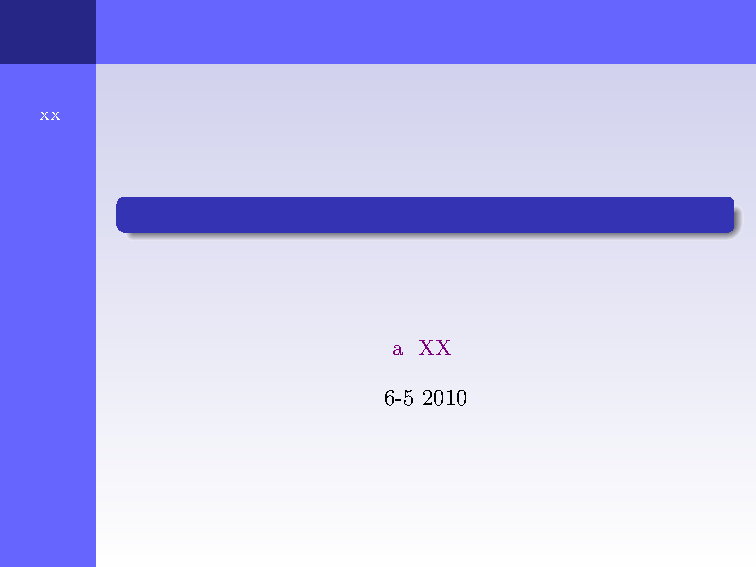
\includegraphics[height=0.09\textwidth]{ustc.eps}}   %左上角科大logo
%%%%%%%%%%%%%%%%%%%%%%%%%%%%%%%%%%%%%%重定义字体、字号命令 %%%%%%%%%%%%%%%%%%%%%%%%%%%%%%%%%%%%%%%%%%%%%%
\newcommand{\songti}{\CJKfamily{song}}        % 宋体
\newcommand{\fangsong}{\CJKfamily{fs}}        % 仿宋体
\newcommand{\kaishu}{\CJKfamily{kai}}         % 楷体
\newcommand{\heiti}{\CJKfamily{hei}}          % 黑体
\newcommand{\lishu}{\CJKfamily{li}}           % 隶书
\newcommand{\youyuang}{\CJKfamily{you}}       % 幼圆
\newcommand{\sihao}{\fontsize{14pt}{\baselineskip}\selectfont}      % 字号设置
\newcommand{\xiaosihao}{\fontsize{12pt}{\baselineskip}\selectfont}  % 字号设置
\newcommand{\wuhao}{\fontsize{10.5pt}{\baselineskip}\selectfont}    % 字号设置
\newcommand{\xiaowuhao}{\fontsize{9pt}{\baselineskip}\selectfont}   % 字号设置
\newcommand{\liuhao}{\fontsize{7.875pt}{\baselineskip}\selectfont}  % 字号设置
\newcommand{\qihao}{\fontsize{5.25pt}{\baselineskip}\selectfont}    % 字号设置
%%%%%%%%%%%%%%%%%%%%%%%%%%%%%%%%%%%%%%%%%%%%%%%%%%%%%%%%%%%%%%%%%%%%%%%%%%%%%%%%%%%%%%%%%%%%%%%%%%%%%%%%
%%----------------------- Theorems ---------------------------------------------------------------------
\newtheorem{theorem}{定理}
\newtheorem{definition}{定义}
\newtheorem{lemma}{引理}
%%----------------------------------------------------------------------------------------------------
\title{\heiti 题目}
\author[\textcolor{white}{\songti 作者~XX君}]{{\songti 指导老师~\textcolor{olive}{老师}}\\{\songti 作者~~\textcolor{olive}{作者}}}
\institute{\wuhao \lishu \textcolor{violet}{a大学~~XX系 }}
\date{6-5 2010}

\begin{document}
 \begin{CJK*}{GBK}{kai}

\begin{frame}
	\titlepage
\end{frame}
%任意两行单列线表示一张ppt
%%---------------------------------------------------------------------------------------------------
\begin{frame}
\frametitle{What is SCCP?}
\begin{itemize}
 \item a
 \item b
 \item b
\end{itemize}
\end{frame}
%%---------------------------------------------------------------------------------------------------
\begin{frame}
\frametitle{What is SCCP?}
abc
\end{frame}
%%---------------------------------------------------------------------------------------------------
\begin{frame}
\frametitle{这是介绍}
\begin{itemize}
 \item 这是介绍
\end{itemize}
\end{frame}
%%---------------------------------------------------------------------------------------------------
\begin{frame}\frametitle{定理}
\begin{lemma}[1]
这是一个定理,引理类似。
\end{lemma}
\pause                       % 这里会暂停一下,pagedown会接着出现下面的式子
\begin{displaymath}             %这个不用解释了吧
1+1=2
\end{displaymath}
\begin{equation}
1+1=2
\end{equation}
\end{frame}
%%================================================================================新目录
\section{未尽的思考}
%%---------------------------------------------------------------------------------------------------
\begin{frame}\frametitle{插个图}
\begin{figure}[!htbp]
\centering
%\includegraphics[width=4.00cm,height=2.10cm]{SD.eps}
\caption{一个图}
\end{figure}
\end{frame}
%%---------------------------------------------------------------------------------------------------
%%---------------------------------------------------------------------------------------------------
\begin{frame}\frametitle{插个表}
一个表.
 \begin{table}
  \centering \addtolength{\tabcolsep}{1mm}
 \begin{tabular}{ccccccccc}
   \hline
        & 1 & 2 & 3 & 4 & 5 & 6 & 7 & 8 \\
   \hline
   1 &         &       &          &       &       &       &       &  \\
   2 & $c$     &       &          &       &       &       &       &  \\
   3 & $c$     & $c $  &          &       &       &       &       &  \\
   4 & $a$     & $a,c$ & $a $     &       &       &       &       &  \\
   5 & $a,b,c$ & $a,b$ & $a,b,c$  & $b,c$ &       &       &       &  \\
   6 & $a,c$   & $a,c$ & $a,c$    & $c $  & $b,c$ &       &       &  \\
   7 & $a,b,c$ & $a,b$ & $a,b,c$  & $b,c$ &       & $b,c$ &       &  \\
   8 & $a,c$   & $a,c$ & $a,c$    & $c$   & $b,c$ &       & $b,c$ &  \\
   \hline
 \end{tabular}\label{dismatrix}
 \end{table}
\end{frame}
%%---------------------------------------------------------------------------------------------------
\begin{frame}\frametitle{就这样吧}
就这样吧,遗计。
\end{frame}
%%================================================================================新目录
\section{参考文献}
%%---------------------------------------------------------------------------------------------------
\begin{frame}\frametitle{参考文献}
[1] A\newline
[2] B
\end{frame}
%%%%%%%%%%%%%%%%%%%%%%%%%%%%%%%%%%%%%%%%%%%%%%%%%%%%%%%%%%%%%%%%%%%%%%%%%%%%%%%%%%%%%%%%%%%%%%
\section{致谢}
%%---------------------------------------------------------------------------------------------------
\begin{frame}\frametitle{致谢}
Thanks
\end{frame}
%%%%%%%%%%%%%%%%%%%%%%%%%%%%%%%%%%%%%%%%%%%%%%%%%%%%%%%%%%%%%%%%%%%%%%%%%%%%%%%%%%%%%%%%%%%%%%
\end{CJK*}
\end{document}
